%%%%%%%%%%%%%%
%
%  第二部分 操作教程
%
%%%%%%%%%%%%%%
\section{操作教程}

\subsection{安装与启动}
\par
本软件基于 Python 3.10 及以上版本开发，首次运行前需安装依赖库。推荐在命令行中执行以下步骤：
\begin{enumerate}
	\item 进入项目根目录；
	\item 安装依赖：\texttt{pip install -r requirements.txt}；
	\item 启动程序：\texttt{python main.py}。
\end{enumerate}
% 插入图：系统启动界面
\begin{figure}[htbp]
	\centering
	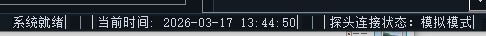
\includegraphics[width=0.8\textwidth]{image/xitong.png}
	\caption{系统启动后界面（显示状态栏、当前时间与探头连接状态）}
	\label{fig:system_startup}
\end{figure}
\par
软件启动后，状态栏显示系统状态、当前时间与探头连接状态（仿真模式）。



\subsection{主界面组成与布局}
\par
软件主界面由菜单栏、工具栏、波形显示区、右侧控制面板、底部频谱分析面板、左侧缺陷统计面板与底部缺陷表格构成，如图2所示。菜单栏包含"文件"、"设置"、"视图"和"帮助"；工具栏提供"打开"、"保存"、"开始检测"、"停止检测"、"冻结"、"单次采样"和"生成报告"；波形显示区展示 A-Scan 曲线，采用黑色背景与绿色网格，支持右键菜单与拖拽交互；右侧控制面板集成检测参数设置、采集控制、闸门设置、定量结果、游标读数和校准入口，当窗口高度不足时会自动出现滚动条；底部缺陷表格用于实时显示当前闸门内的峰值读数，并记录历史缺陷信息。
说明：缺陷表格第1行为"实时行"，用于展示当前闸门内峰值读数，不参与删除；历史记录需在"开始记录"后才会写入。

\par
新增功能面板（可通过"视图"菜单或快捷键显示/隐藏）：
\begin{enumerate}
	\item 频谱分析面板（F5）：位于界面底部，提供 FFT 频谱分析、数字滤波器功能，详见第2.10节；
	\item 缺陷统计面板（F6）：位于界面左侧，提供缺陷统计分析、DAC 曲线显示功能，详见第2.11节。
\end{enumerate}

% 插入图：主界面整体截图
\begin{figure}[htbp]
	\centering
	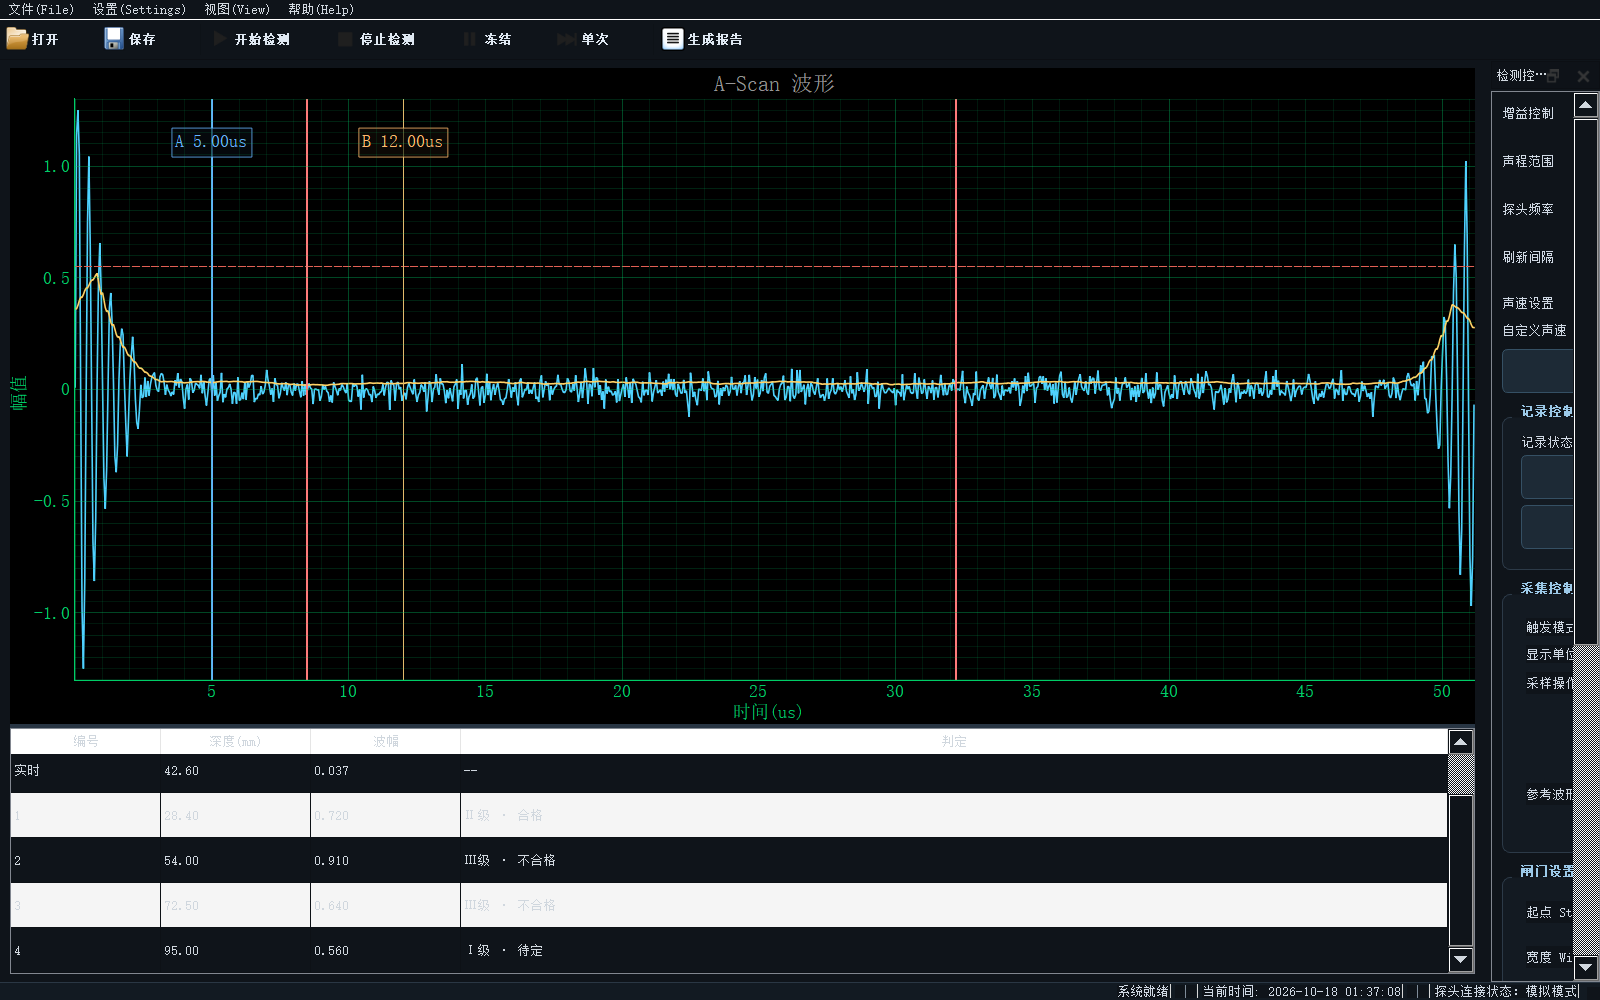
\includegraphics[width=0.95\linewidth]{image/ui_main.png}
	\caption{主界面整体（含新增频谱分析面板与缺陷统计面板入口）}
	\label{fig:ui_main}
\end{figure}

% 插入图：频谱分析面板截图
\begin{figure}[htbp]
	\centering
	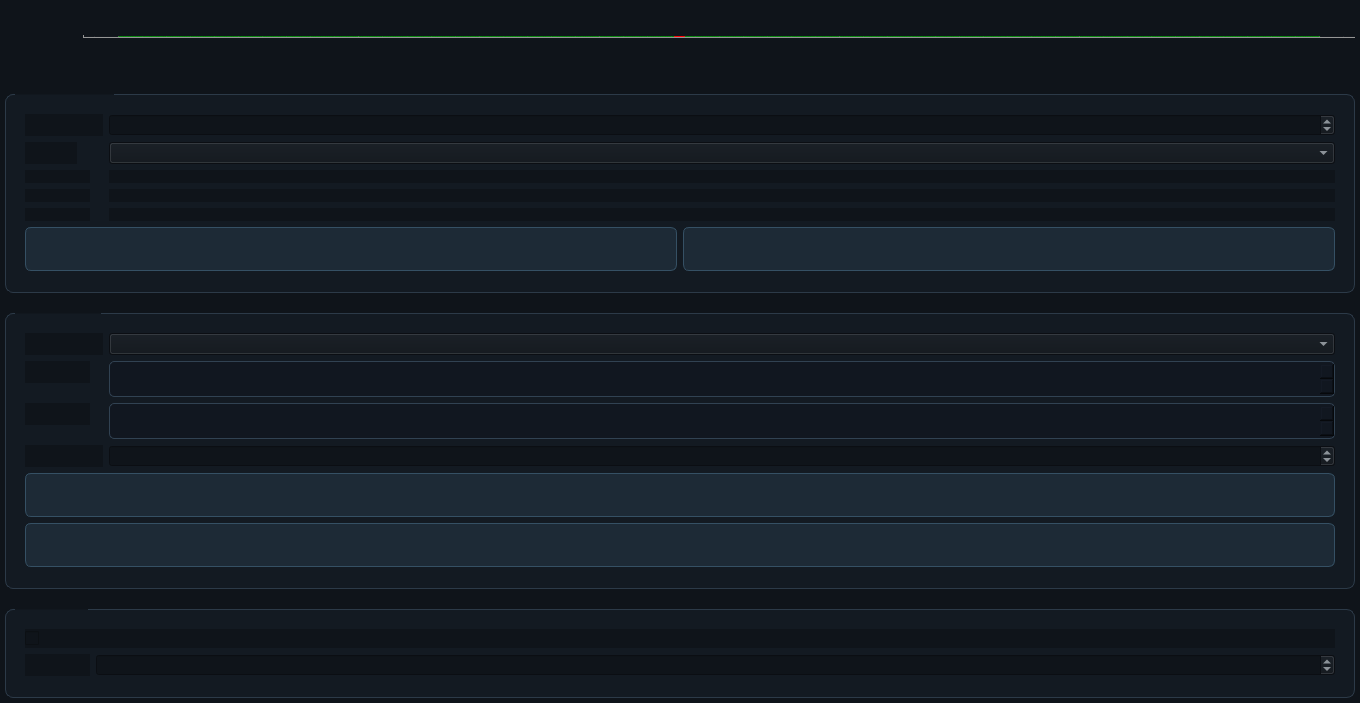
\includegraphics[width=0.95\linewidth]{image/fft_panel.png}
	\caption{频谱分析面板（FFT 频谱图、窗函数选择、数字滤波器）}
	\label{fig:fft_panel}
\end{figure}

% 插入图：缺陷统计面板截图
\begin{figure}[htbp]
	\centering
	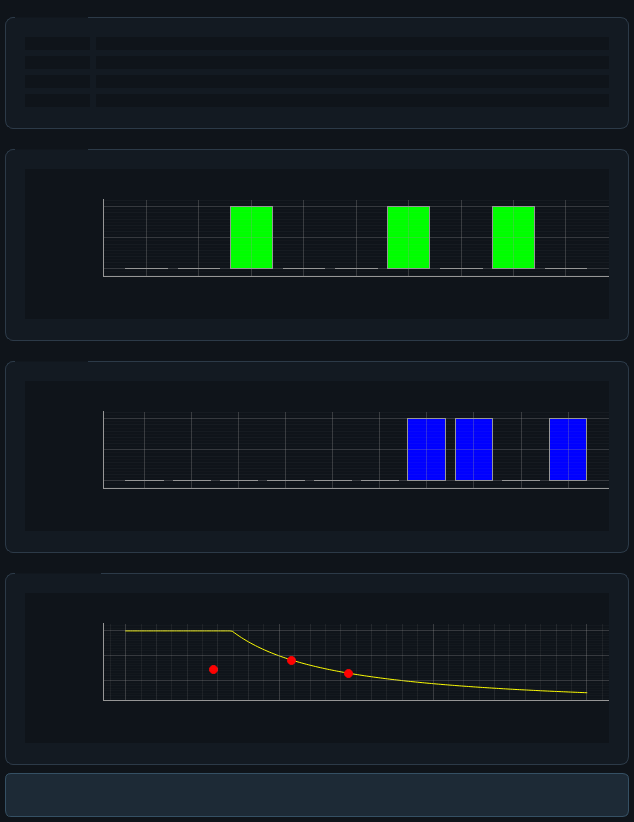
\includegraphics[width=0.95\linewidth]{image/statistics_panel.png}
	\caption{缺陷统计面板（统计数据、深度/波幅分布图、DAC 曲线）}
	\label{fig:statistics_panel}
\end{figure}
\FloatBarrier



\subsection{检测参数设置}
\par
常用检测参数位于右侧控制面板，建议按以下顺序配置：
\begin{enumerate}
	\item 增益（Gain）：范围 0$\sim$110 dB，用于调节整体波幅；
	\item 声程范围（Range）：0$\sim$500 mm，用于设置显示/检测的最大范围；
	\item 探头频率（Frequency）：仿真信号中心频率（默认 2.5 MHz）；
	\item 刷新间隔（Refresh）：采集刷新周期，数值越大，波形更新越慢，便于观察；
	\item 声速（Velocity）：可选择钢（5900 m/s）、铝（6300 m/s）或自定义，用于深度换算。
\end{enumerate}
\par
参数修改后，点击"应用参数"使其生效。

\subsection{采集控制（开始/停止/冻结/单次）}
\par
采集控制用于管理波形刷新与显示行为：
\begin{enumerate}
	\item 开始检测：启动定时采集并刷新波形；
	\item 停止检测：停止采集刷新；
	\item 冻结：暂停显示更新，用于精读当前波形（不改变参数配置）；
	\item 单次采样：在冻结或停止状态下获取一帧波形并显示；
	\item 触发模式：
	\begin{enumerate}
		\item 自动：按刷新周期持续更新；
		\item 闸门触发：仅当闸门触发条件满足时更新（模拟触发采样）。
	\end{enumerate}
	\item 峰值保持：对波形峰值进行保持显示，便于观察上包络变化；
	\item 参考波形：可捕获一条参考曲线用于对比，必要时可清除。
\end{enumerate}
\par
若用户发现波形"无变化"，请优先检查是否处于冻结状态，或触发模式设置为"闸门触发"但当前未触发。

\subsection{闸门（Gate A）设置与使用}
\par
闸门用于在指定窗口内进行峰值检测与报警/记录。本软件采用常见的 Start/Width/Level 三参数线性闸门：
\begin{enumerate}
	\item Start：闸门起点（对应波形时间或深度轴上的起始位置）；
	\item Width：闸门宽度（闸门终点 = Start + Width）；
	\item Level：门限高度（以屏高比例表示，用于触发判定）。
\end{enumerate}
\par
一条\textbf{可拖拽横线}表示门限。用户可在右侧输入框中精确输入 Start/Width/Level，也可直接在图上拖拽调整，二者会自动联动。
\par
闸门检测逻辑为：在闸门窗口内搜索最大波峰值（Peak），当 Peak 超过门限时，波形图会用红色圆点标记峰值位置，并在右侧更新定量结果（深度、水平距离、dB 差值等）。界面效果如图3所示。

\begin{figure}[htbp]
	\centering
	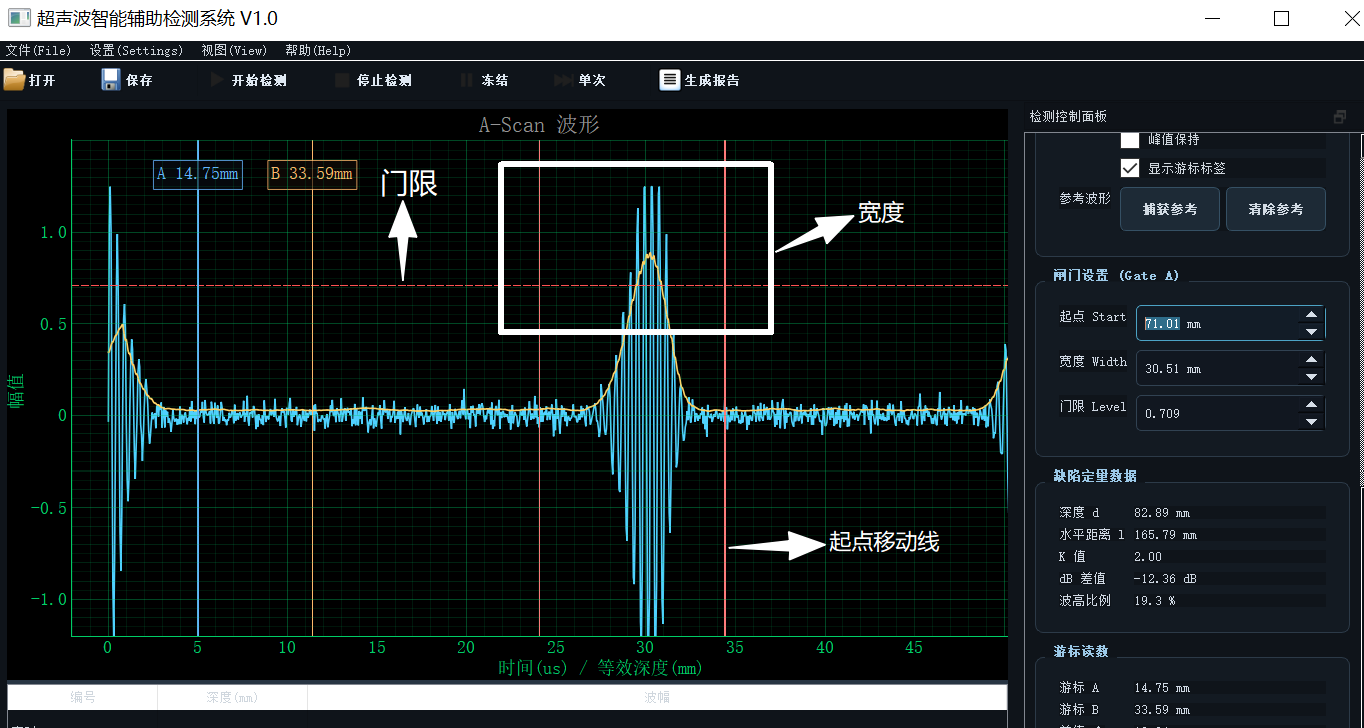
\includegraphics[width=0.95\linewidth]{image/gate_lines.png}
	\caption{阀门线（Start/End/Level）}
\end{figure}

\subsection{游标 A/B 测量}
\par
游标用于读取波形指定位置的时间/深度与幅度。本软件提供两条可拖拽竖线游标 A、B：
\begin{enumerate}
	\item 在波形图中拖动游标 A/B 可改变位置；
	\item 右侧面板实时显示 A、B 的读数及差值 $\Delta$；
	\item 可在"视图"菜单或右侧开关中控制"显示游标标签"；
	\item 游标标签固定显示在图形高度约 90\% 处，避免遮挡波形细节。
\end{enumerate}

\par
如图\ref{fig:cursor_ab}所示，游标 A 和 B 分别以蓝色和橙色竖线标记在波形图上，右侧控制面板同步显示其位置及差值信息。

\begin{figure}[htbp]
	\centering
	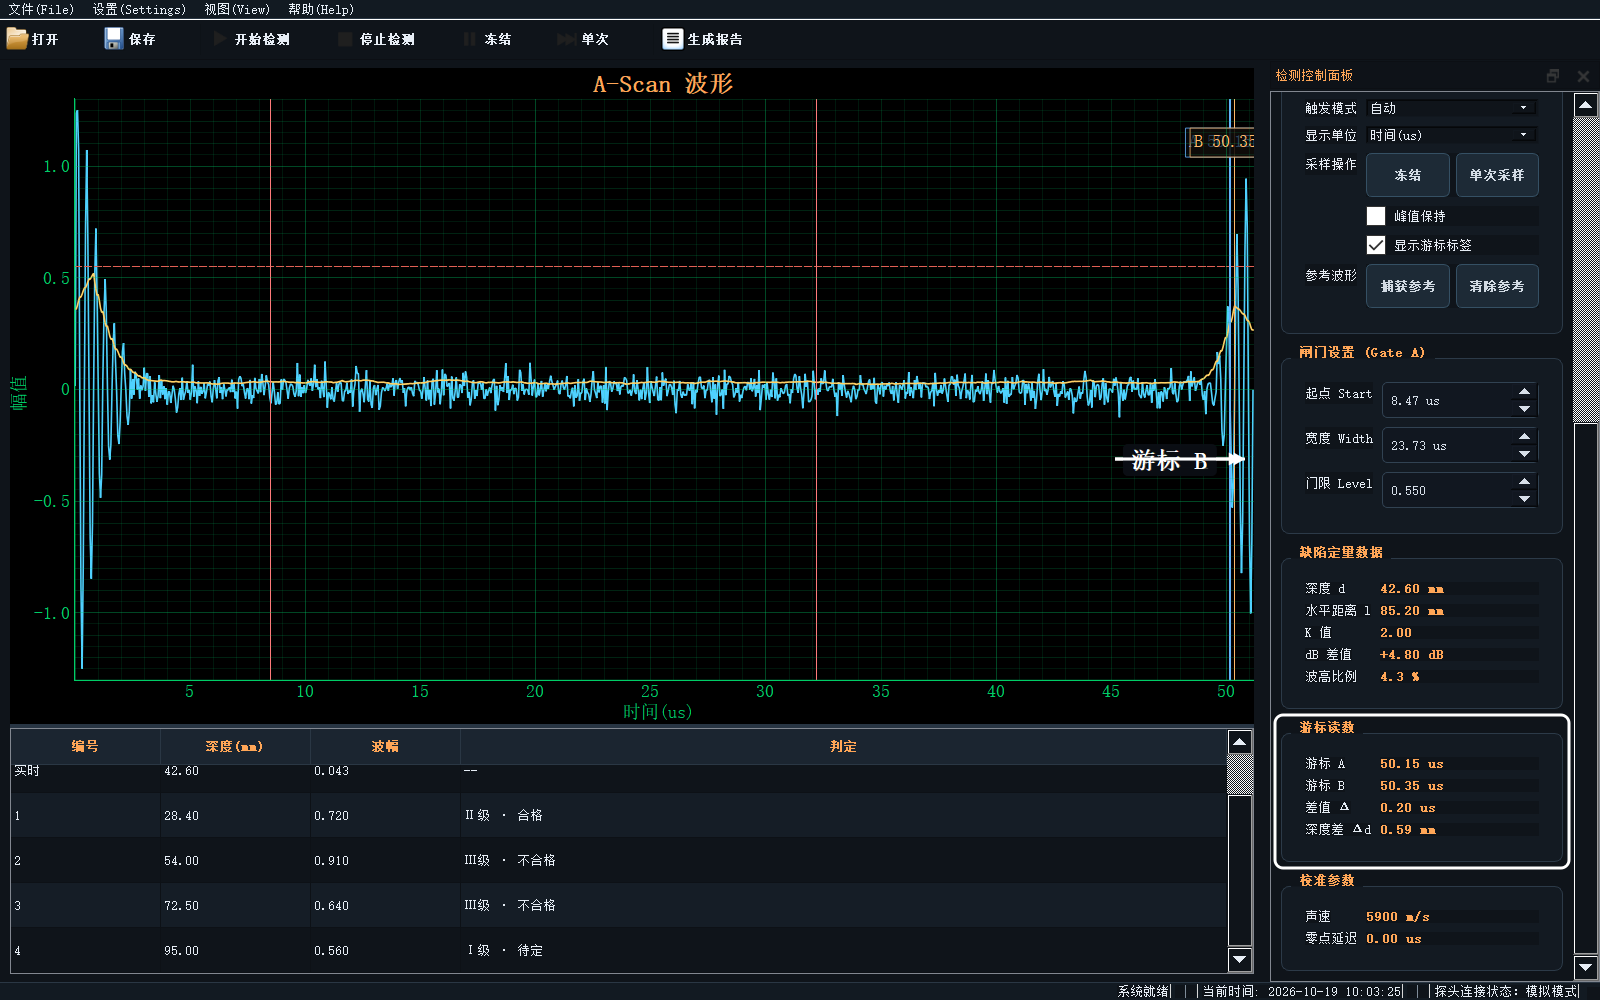
\includegraphics[width=0.95\linewidth]{image/cursor_ab.png}
	\caption{游标 A/B 与读数区域}
	\label{fig:cursor_ab}
\end{figure}
\FloatBarrier

\subsection{缺陷记录与表格管理}
\par
缺陷记录用于形成可追溯数据，避免"误触发即入表"的不合理行为。本软件采用"手动开始记录"的方式：
\begin{enumerate}
	\item 点击"开始记录"后，闸门触发事件会写入历史记录；
	\item 未开始记录时，仅更新表格实时行，不写入历史；
	\item 右键缺陷表格可执行：删除选中、清空历史、重编号等操作；
	\item 实时行不可删除，历史行支持键盘 Delete 删除。
\end{enumerate}

% 插入图4：缺陷表格与右键菜单
\begin{figure}[htbp]
	\centering
	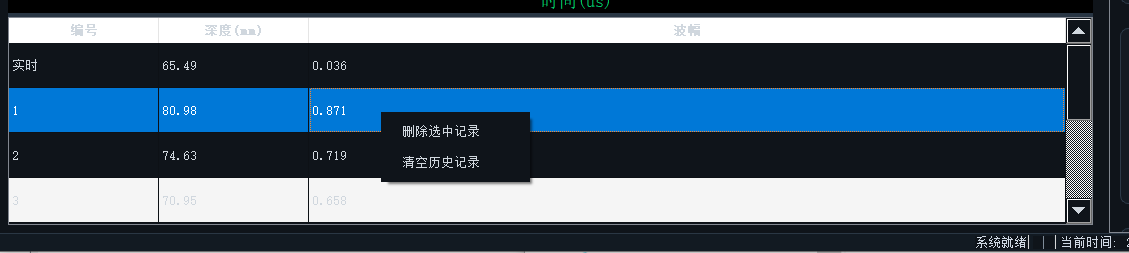
\includegraphics[width=0.95\textwidth]{image/defect.png}
	\caption{缺陷记录表格及右键上下文菜单}
	\label{fig:defect_table_menu}
\end{figure}

\subsection{数据保存与导出}
\par
点击"保存"可将当前波形数据与参数导出为 JSON 或 CSV 文件：
\begin{enumerate}
	\item JSON：包含参数信息与完整数组（时间序列、原始波形、包络/保持等）；
	\item CSV：以表格形式保存时间与幅度数据，便于在第三方软件中分析。
\end{enumerate}
\par
点击"打开"可选择历史数据文件并进行提示（波形回放/复现属于后续可扩展能力）。

\subsection{报告生成与判定规则}
\par
点击"生成报告"将弹出报告预览窗口，并可保存为 HTML 文件。报告预览窗口如图6所示，报告内容包含：

% 插入图5：报告预览窗口
\begin{figure}[htbp]
	\centering
	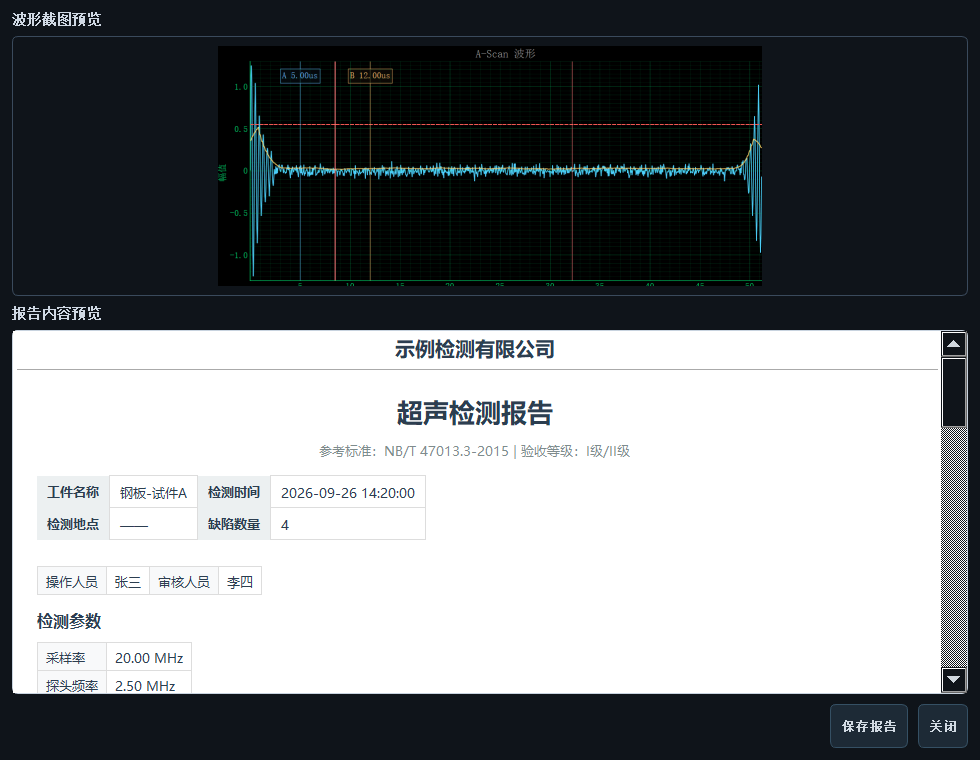
\includegraphics[width=0.90\textwidth]{image/report_preview.png}
	\caption{报告预览窗口}
	\label{fig:report_preview}
\end{figure}
\begin{enumerate}
	\item 检测时间、工件名称（当前默认"工件-001"）与基础参数；
	\item 参考标准与验收等级（支持通用、NB/T 47013、GB/T 11345、ASME 等标准模板）；
	\item 检测人员信息（操作人员、审核人员、公司名称、检测地点等，可选填）；
	\item 检测参数自动嵌入（采样率、探头频率、增益、声速、扫查深度等）；
	\item 当前波形总览截图；
	\item 每条缺陷记录对应的波形截图（用于追溯）。
\end{enumerate}

% 插入图6：完整报告
\begin{figure}[htbp]
	\centering
	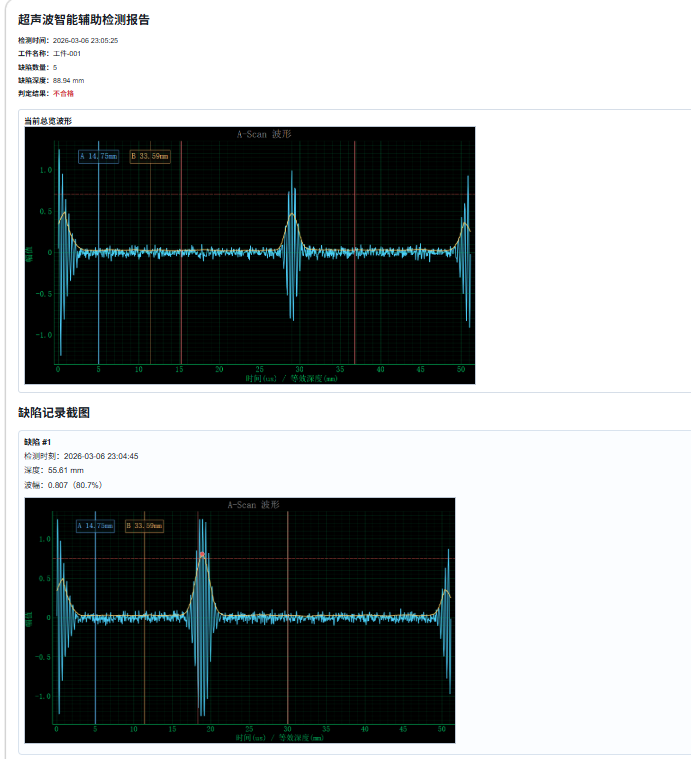
\includegraphics[width=0.90\textwidth]{image/report.png}
	\caption{完整报告}
	\label{fig:complete_report}
\end{figure}
\par
判定规则：当存在缺陷记录，或当前帧闸门触发时，判定为"不合格"；否则判定为"合格"。此规则保证报告结论与记录数据一致，避免"有缺陷但合格"的逻辑矛盾。
\FloatBarrier

\subsection{校准功能（声速与零点）}
\par
为提升读数准确性，软件提供两类校准：
\begin{enumerate}
	\item 声速校准：根据已知厚度与实测往返时间推算声速；
	\item 零点校准：对系统零点延迟进行补偿，改善浅表读数。
\end{enumerate}
% 插入图7：校准功能界面截图
\begin{figure}[htbp]
	\centering
	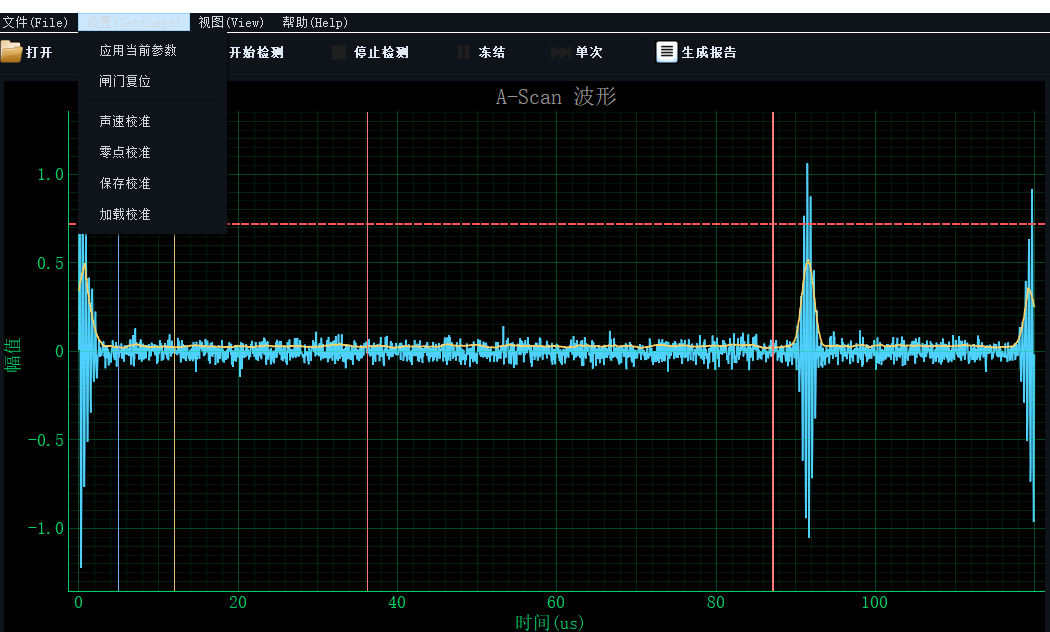
\includegraphics[width=0.95\textwidth]{image/calibration_menu.png}
	\caption{校准功能界面（包含声速校准、零点校准等选项）}
	\label{fig:calibration_menu}
\end{figure}
\par
校准功能界面如图8所示，校准参数支持保存/加载（JSON），便于不同材料/工件快速切换。
\FloatBarrier

\subsection{鼠标右键菜单（波形区）}
% 插入图8：波形区右键菜单界面截图
\begin{figure}[htbp]
	\centering
	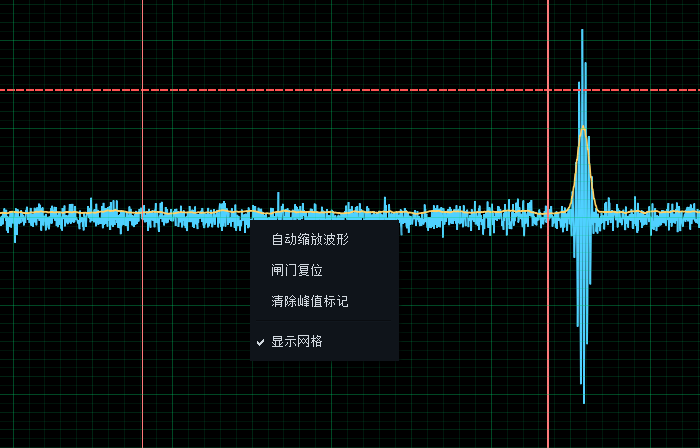
\includegraphics[width=0.95\textwidth]{image/context_menu_waveform.png}
	\caption{波形区右键菜单界面（包含自动缩放、闸门复位、清除峰值标记等功能）}
	\label{fig:context_menu_waveform}
\end{figure}
\par
在波形图区域点击鼠标右键，可打开中文快捷菜单（例如：自动缩放、闸门复位、清除峰值标记、显示网格开关等），用于提升操作效率，菜单界面如图9所示：
\FloatBarrier

\subsection{频谱分析功能（新增）}
\par
频谱分析功能用于在频率域观察超声信号特性，帮助用户识别信号中的主要频率成分和噪声分布。该功能通过界面底部的"频谱分析面板"实现（按 F5 键或通过"视图"菜单显示/隐藏）。

\subsubsection{FFT 频谱分析}
\par
在频谱分析面板中，点击"计算 FFT"按钮即可对当前 A-Scan 波形执行快速傅里叶变换，并在面板中显示频谱图。可调参数包括：
\begin{enumerate}
	\item FFT 点数：256$\sim$8192，数值越大频率分辨率越高，但计算量增大；
	\item 窗函数：矩形窗、汉宁窗、汉明窗、布莱克曼窗，不同窗函数对频谱泄漏的抑制效果不同。
\end{enumerate}
\par
频谱图自动标注峰值频率（单位 MHz）和峰值幅值（单位 dB），便于用户快速定位信号主频。

\subsubsection{数字滤波器}
\par
频谱分析面板提供三种数字滤波器，用于对当前波形进行频率选择性滤波：
\begin{enumerate}
	\item 带通滤波器：仅保留指定频率范围内的信号成分；
	\item 低通滤波器：滤除高频噪声，保留低频信号；
	\item 高通滤波器：滤除低频干扰（如始波附近的低频振铃），保留高频缺陷回波。
\end{enumerate}
\par
参数说明：
\begin{enumerate}
	\item 低频截止 / 高频截止：单位 MHz，可精确设定滤波频率边界；
	\item 滤波器阶数：1$\sim$10，阶数越高过渡带越窄，但可能引入更多振铃。
\end{enumerate}
\par
点击"应用滤波器"后，滤波结果会实时更新到 A-Scan 波形图上。

% 插入图：频谱分析面板截图
\begin{figure}[htbp]
	\centering
	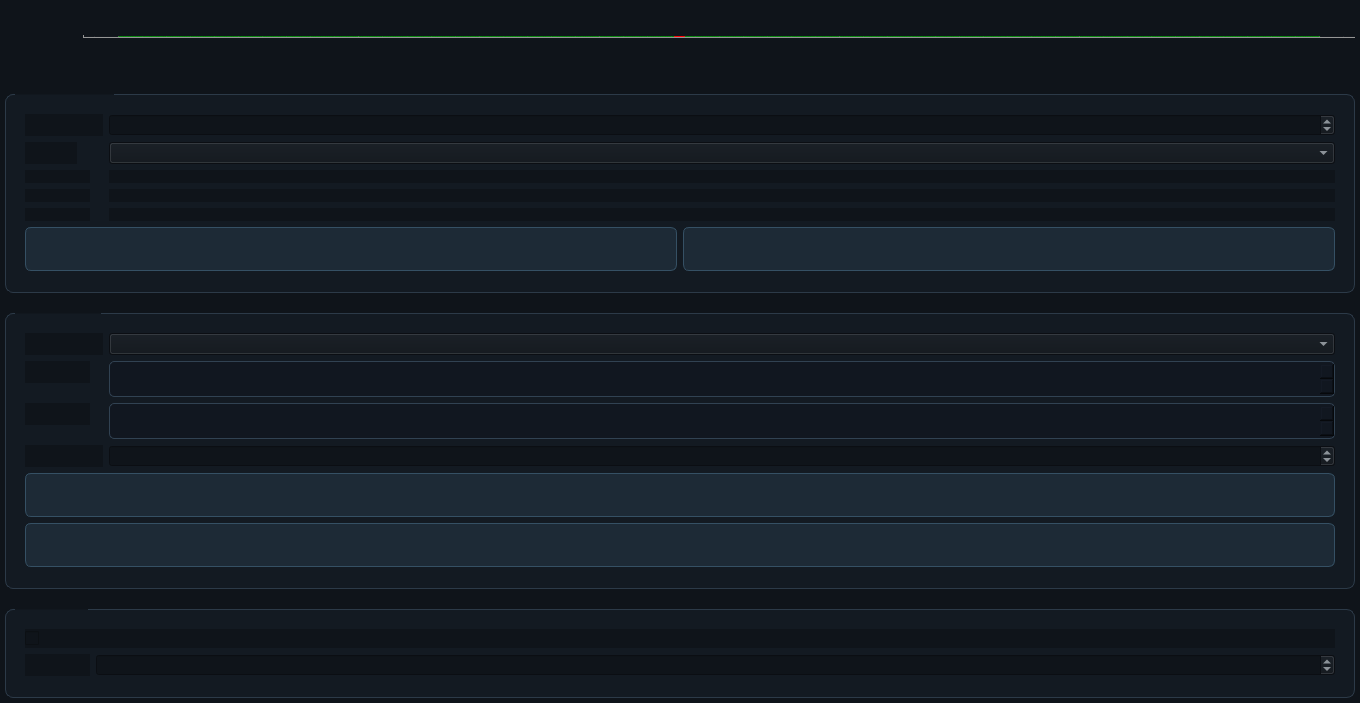
\includegraphics[width=0.95\linewidth]{image/fft_panel.png}
	\caption{频谱分析面板（FFT 频谱图、数字滤波器控制）}
	\label{fig:fft_panel_detail}
\end{figure}
\FloatBarrier

\subsection{缺陷统计分析功能（新增）}
\par
缺陷统计分析功能用于对已记录的缺陷进行统计汇总和可视化展示，帮助用户评估缺陷分布规律。该功能通过界面左侧的"缺陷统计面板"实现（按 F6 键或通过"视图"菜单显示/隐藏）。

\subsubsection{统计数据}
\par
面板顶部显示缺陷统计摘要：
\begin{enumerate}
	\item 缺陷总数：已记录的缺陷数量；
	\item 深度范围：缺陷深度的最小值与最大值（单位 mm）；
	\item 平度深度：所有缺陷深度的算术平均值；
	\item 平均波幅：所有缺陷波幅的算术平均值（以屏高百分比表示）。
\end{enumerate}

\subsubsection{分布图}
\par
面板中部以柱状图形式展示缺陷的深度分布和波幅分布：
\begin{enumerate}
	\item 深度分布：按 10 mm 区间统计缺陷数量，便于判断缺陷集中区域；
	\item 波幅分布：按 10\% 区间统计缺陷数量，便于评估缺陷严重程度。
\end{enumerate}

\subsubsection{DAC 曲线}
\par
面板底部显示距离-波幅校正曲线（DAC 曲线），用于缺陷定量评估：
\begin{enumerate}
	\item DAC 曲线基于超声衰减原理自动生成，波幅随深度增加而减小；
	\item 已记录的缺陷以红色圆点标注在图上，便于与 DAC 曲线对比；
	\item 可快速判断缺陷是否超过验收标准对应的 DAC 门限。
\end{enumerate}
\par
点击"刷新统计"按钮可更新统计数据和图表。

% 插入图：缺陷统计面板截图
\begin{figure}[htbp]
	\centering
	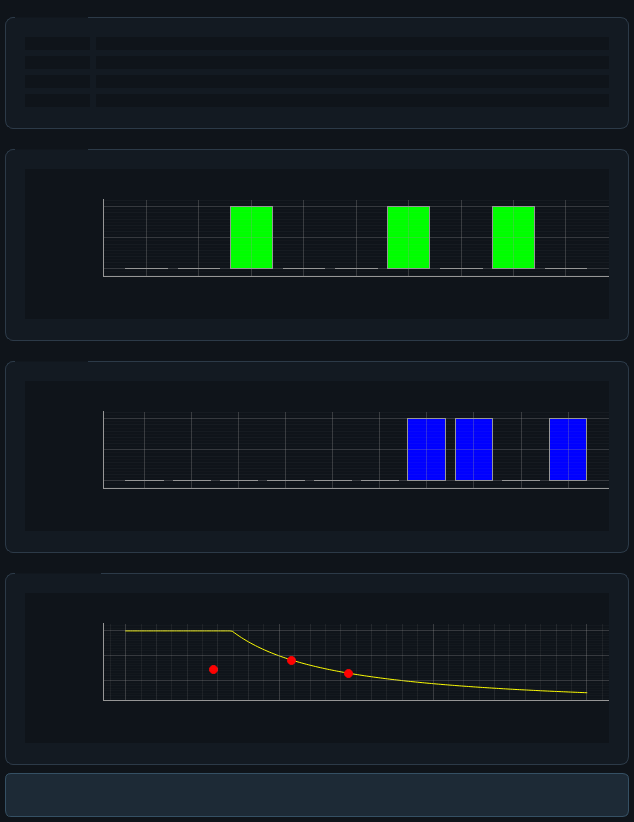
\includegraphics[width=0.95\linewidth]{image/statistics_panel.png}
	\caption{缺陷统计面板（统计数据、深度/波幅分布图、DAC 曲线）}
	\label{fig:statistics_panel_detail}
\end{figure}
\FloatBarrier

\subsection{快捷键系统（新增）}
\par
为提高操作效率，本软件提供完整的快捷键支持。用户可通过"帮助"菜单中的"快捷键帮助"（或按 F1）查看所有快捷键一览表。常用快捷键如下：

\begin{table}[htbp]
	\centering
	\caption{常用快捷键一览}
	\label{tab:shortcuts}
	\begin{tabular}{|l|l|}
		\hline
		\textbf{快捷键} & \textbf{功能} \\
		\hline
		F1 & 显示快捷键帮助 \\
		\hline
		F2 & 停止检测 \\
		\hline
		F3 & 冻结/解冻波形 \\
		\hline
		F4 & 单次采样 \\
		\hline
		F5 & 显示/隐藏频谱分析面板 \\
		\hline
		F6 & 显示/隐藏缺陷统计面板 \\
		\hline
		Ctrl+O & 打开数据文件 \\
		\hline
		Ctrl+S & 保存波形数据 \\
		\hline
		Ctrl+R & 生成检测报告 \\
		\hline
		Ctrl+A & 自动缩放波形 \\
		\hline
		Ctrl+G & 捕获参考波形 \\
		\hline
		Ctrl+L & 显示/隐藏游标标签 \\
		\hline
		Delete & 删除选中的缺陷记录 \\
		\hline
	\end{tabular}
\end{table}

\par
此外，软件支持界面布局记忆功能：窗口位置、大小和面板停靠状态会在关闭时自动保存，下次启动时自动恢复，无需每次重新调整。

\subsection{常见问题}
\par
以下为常见问题与处理建议：
\begin{enumerate}
	\item 波形不更新：检查是否点击"开始检测"、是否处于"冻结"、触发模式是否为"闸门触发"且未触发；
	\item 刷新过快看不清：增大"刷新间隔"，或使用"冻结+单次采样"组合；
	\item 表格无法删除：实时行不可删，请选中历史行再删除或使用"清空历史"；
	\item 报告无法打开：本软件导出为 HTML 文本文件，可直接用浏览器打开（避免二进制不可读问题）；
	\item FFT 频谱图无显示：请先点击"开始检测"或执行"单次采样"获取波形数据，再点击"计算 FFT"；
	\item 滤波器效果不明显：尝试调整截止频率和滤波器阶数，或切换滤波器类型（带通/低通/高通）；
	\item 缺陷统计面板无数据：请先进行缺陷记录（点击"开始记录"并触发缺陷），再点击"刷新统计"；
	\item 快捷键不响应：确认当前焦点不在输入框内（输入框内键盘输入会被优先处理）；
	\item 界面布局错乱：删除安装目录下的 \texttt{config/layout.json} 文件后重启软件，即可恢复默认布局。
\end{enumerate}
